\section{Auswertung}
\label{sec:Auswertung}
\subsection{Statische Methode}
\begin{figure}
  \centering
  \caption{Temperaturverläufe im statischen Fall}
\begin{subfigure}{0.48\textwidth}
  \centering
  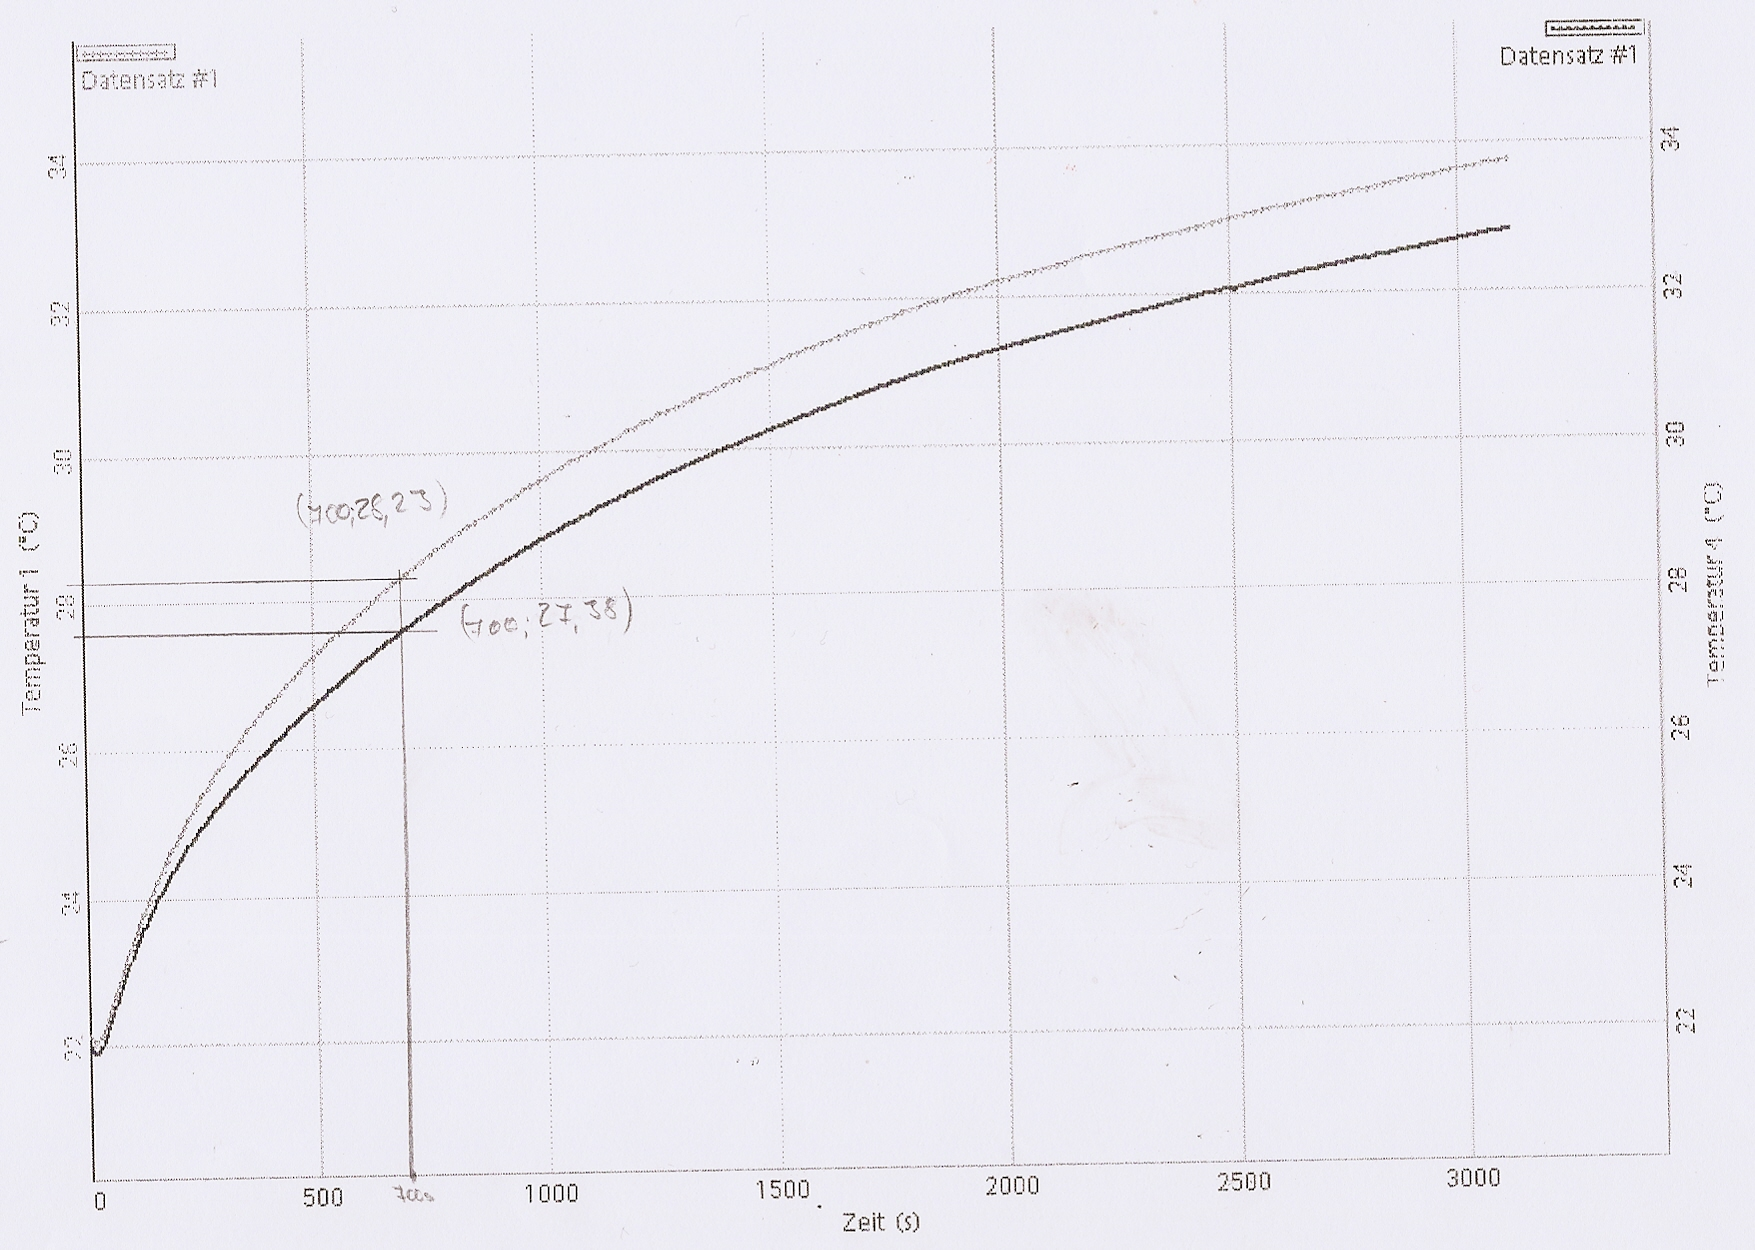
\includegraphics[height= 5cm]{logos/T1T4.jpg}
  \caption{von Termoelement 1 (Messing breit,grau) und 4 (Messsing schmal,schwarz)}
  \label{fig:t1t4}
\end{subfigure}
\begin{subfigure}{0.48\textwidth}
  \centering
  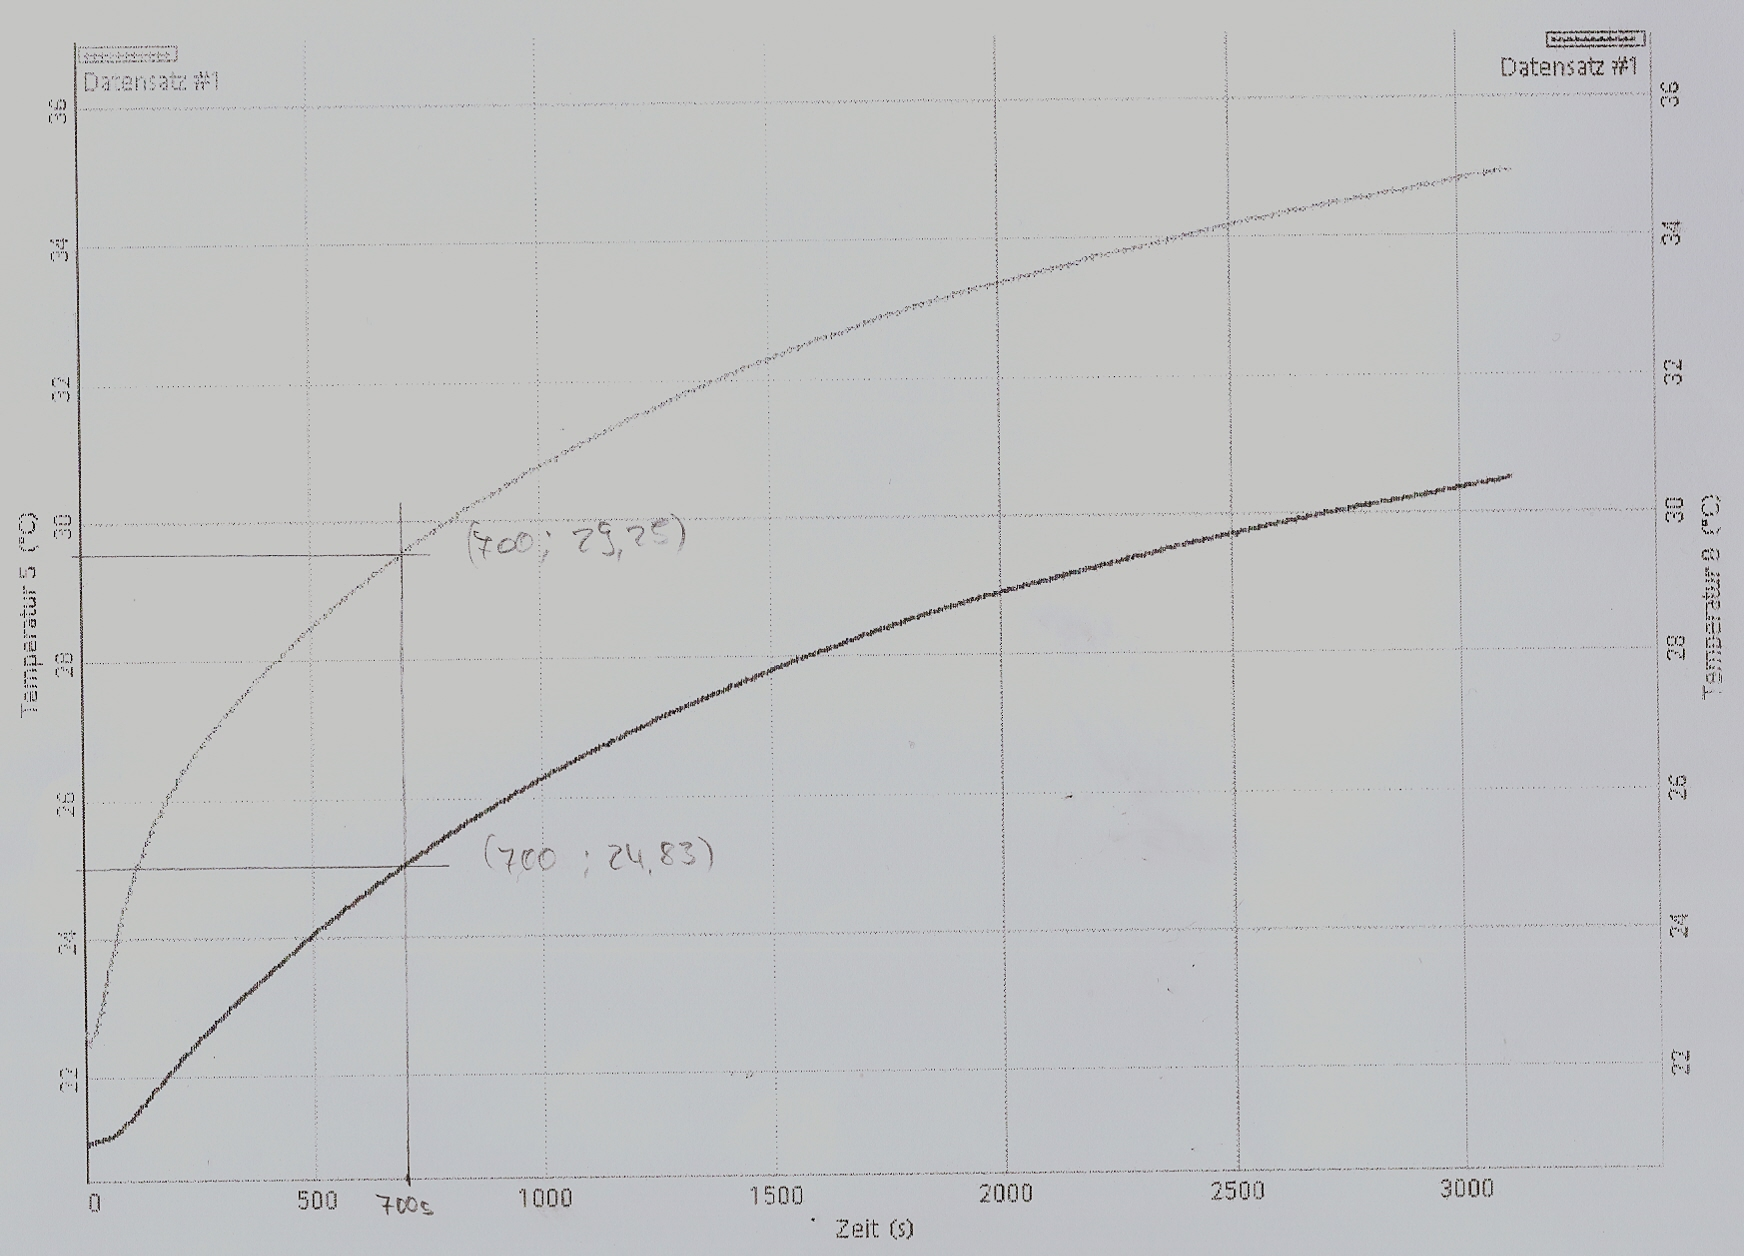
\includegraphics[height= 5cm]{logos/T5T8.jpg}
  \caption{von Termoelement 5 (Aluminium,grau) und 8 (Stahl,schwarz)}
  \label{fig:t5t8}
\end{subfigure}
\label{fig:sfall}
\end{figure}
Alle Temperaturverläufe zeigen die selbe Form des Anstieges (s.Abb.
\ref{fig:sfall}). Der Unterschied besteht
nur darin, wie stark der Anstieg für das jeweilige Element ist. Das lässt sich
gut vergleichen in dem die Temperatur nach einer bestimmten Zeit bei gleichen
Bedingungen für jedes Element gemessen wird. Das ist in der Tabelle \ref{tab:700s}
dargestellt. Daraus kann man erkennen, dass Aluminium den stärksten Anstieg und
somit die bessere Wärmeleitung hat.
\begin{table}
  \centering
  \caption{Temperaturen nach 700s bei der statischen Methode}
  \begin{tabular}{c c}
    \toprule
    Metal & Temperatur in \si{\celsius} \\
    \midrule
    Messing (schmal) & 27,38 \\
    Messing (breit) & 28,23 \\
    Aluminium & 29,25 \\
    Stahl & 24,83 \\
    \bottomrule
  \end{tabular}
  \label{tab:700s}
\end{table}
\FloatBarrier
In Abbildung \ref{fig:dt} sind die Temperaturdifferenzen im Zeitlichenverlauf zu
sehen. Beide Graphen zeigen, dass sich die Differenzen einem Wert annähren und
diesen dann bei behalten, also nach einer Zeit konstant sind.
Der Unterschied zwischen Abbildung \ref{fig:dt2t1} und \ref{fig:dt7t8} ist, dass
der Graph von \ref{fig:dt2t1} einen Peak im Anfang der Messung zeigt, sich also von
oben einem konstanten Wert annährt.
\begin{figure}
  \centering
  \caption{Zeitlicherverlauf der Temperaturdifferenzen}
  \begin{subfigure}{0.48\textwidth}
    \centering
    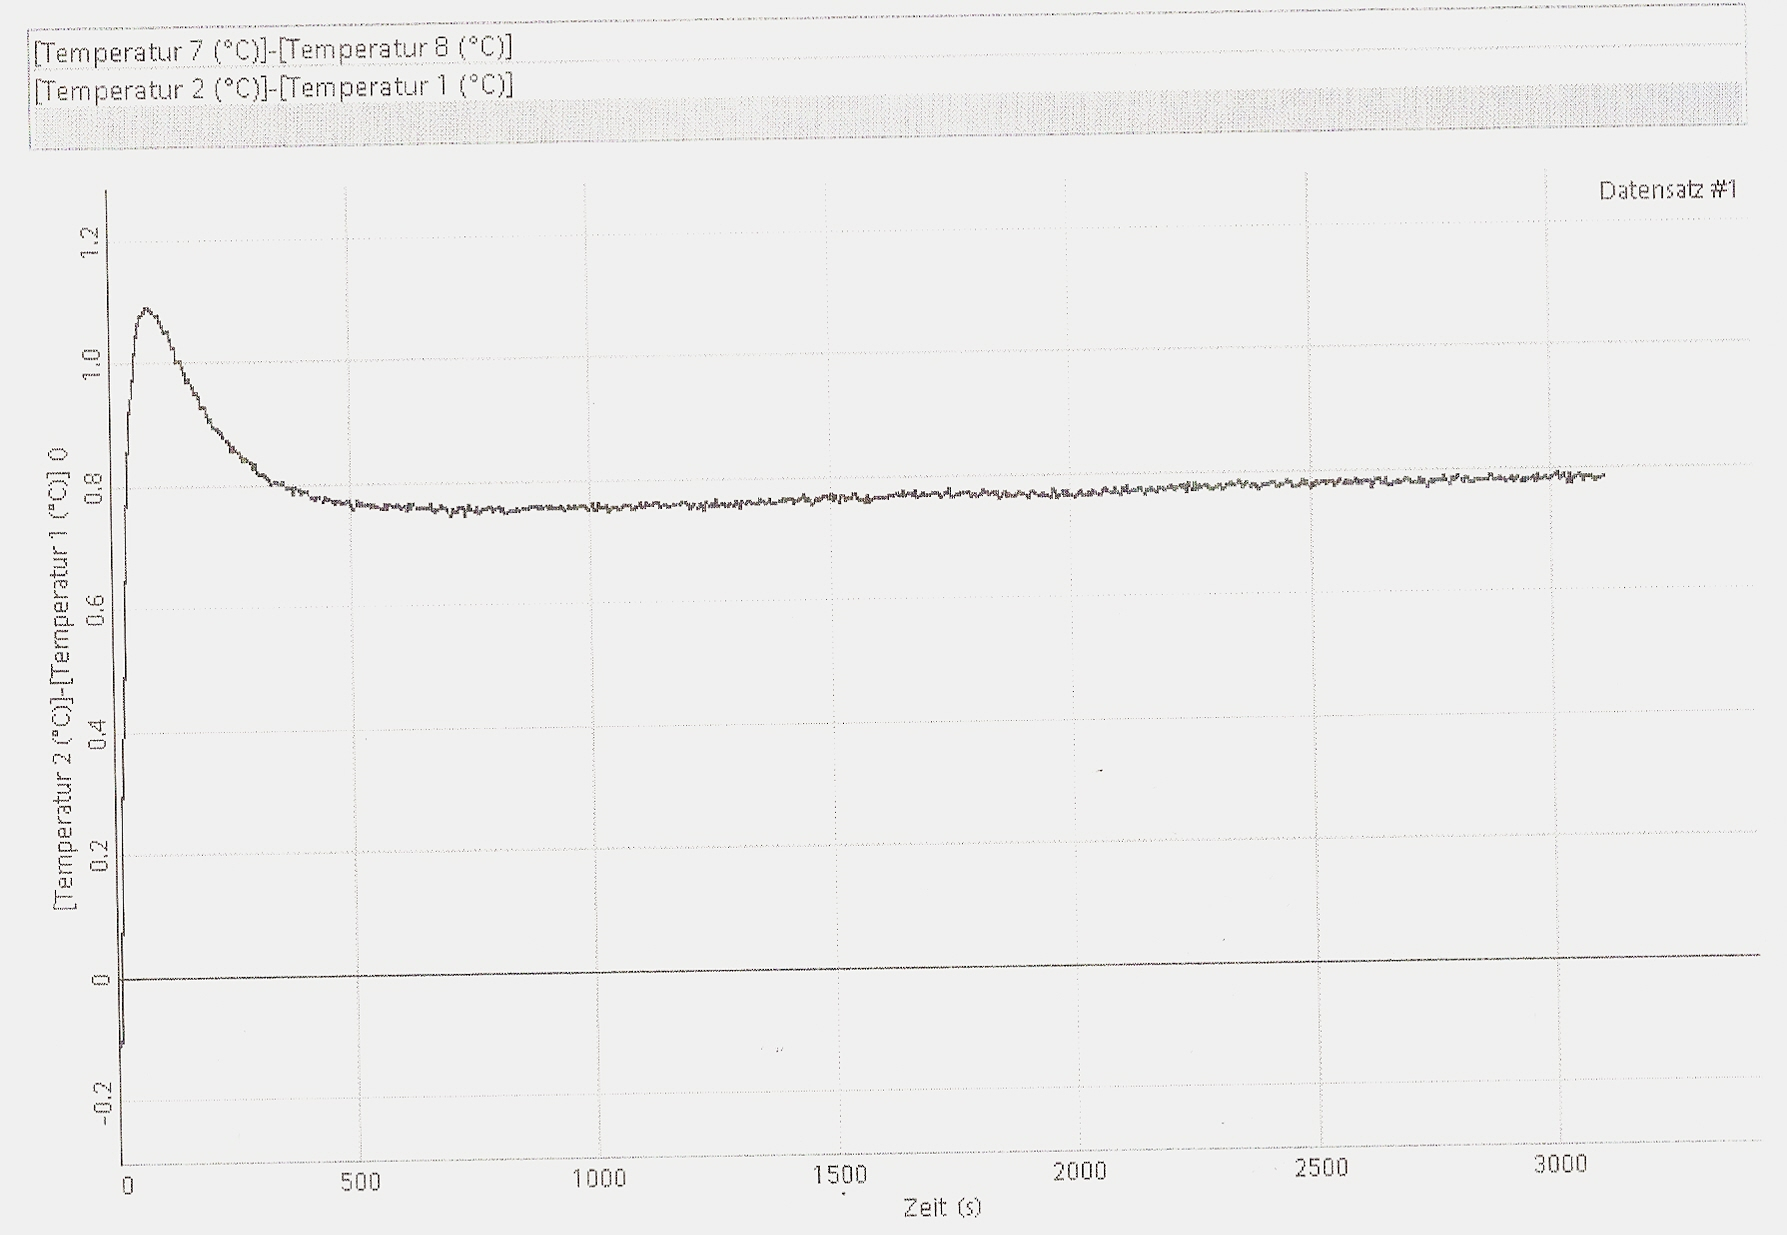
\includegraphics[height = 5cm, width = \textwidth]{logos/T2-T1.jpg}
    \caption{von Termoelement 2 und 1 (Messing breit)}
    \label{fig:dt2t1}
  \end{subfigure}
  \begin{subfigure}{0.48\textwidth}
    \centering
    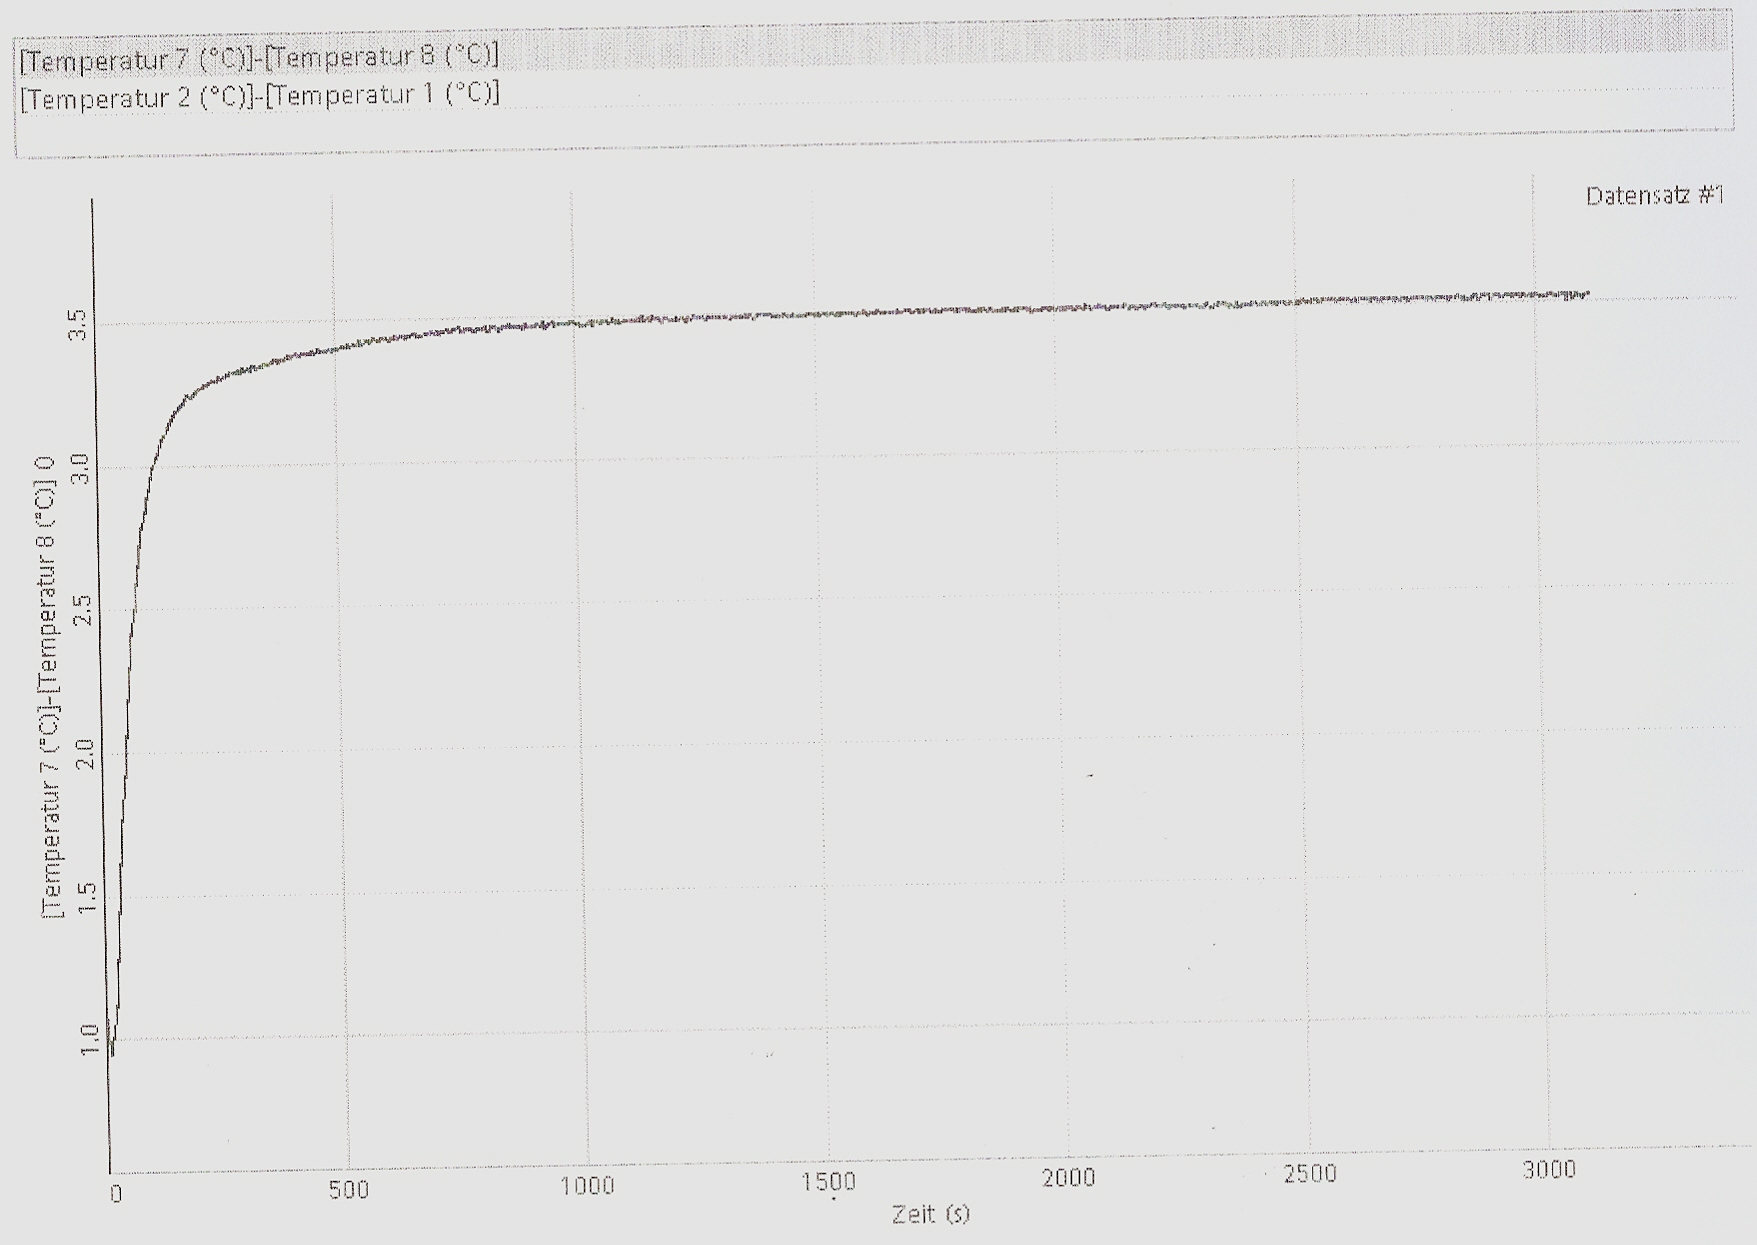
\includegraphics[height=5cm, width = \textwidth]{logos/T7-T8.jpg}
    \caption{von Termoelement 7 und 8 (Edelstahl)}
    \label{fig:dt7t8}
  \end{subfigure}
  \label{fig:dt}
\end{figure}
Aus den Werten von Abbildung \ref{fig:dt} kann mit der Gleichung
\begin{equation*}
  \frac{\increment Q}{\increment t} =
  - \kappa A \frac{\increment T}{\increment x}
\end{equation*}
der Wärmestrom zwischen den Termoelementen bestimmt werden. Dabei bezeichnet
$\frac{\increment Q}{\increment t}$ den Wärmestrom, $\kappa$ die Wärmeleitfähigkeit,
$A$ die Querschnittsfläche, $\increment T$ die Temperaturdifferenz auf dem
Leiterstück $\increment x$ zwischen den Termoelementen. Die Wärmeleitfähigkeit
$\kappa$ wurde für Messing mit 120 \si{\watt\per\meter\per\kelvin}, für
Aluminium mit 236 \si{\watt\per\meter\per\kelvin} ud für Stahl mit 58
\si{\watt\per\meter\per\kelvin} angenommen \cite{wiki}.
\begin{table}
  \centering
  \caption{Berechneter Wärmestrom}
  \sisetup{round-mode = places , round-precision = 2}
  \begin{tabular}{S[table-figures-decimal=0] S S S S}
    \toprule
    t/\si{\second} & $\increment T_{Messing}$ / \si{\celsius}
    & $\frac{\increment Q_{Messing}}{\increment t}$ / \si{\watt}
    &$\increment T_{Edelstahl}$ / \si{\celsius}
    &$\frac{\increment Q_{Edelstahl}}{\increment t}$ / \si{\watt} \\
    \midrule
    250 & 3.299999999999999822e+00 & -6.336000000000000520e-01 & 8.599999999999999867e-01 & -7.980800000000000394e-02\\
    500 & 3.390000000000000124e+00 & -6.508800000000001251e-01 & 7.600000000000000089e-01 & -7.052800000000000735e-02\\
    750 & 3.459999999999999964e+00 & -6.643200000000001326e-01 & 7.500000000000000000e-01 & -6.959999999999999520e-02\\
    1000 & 3.470000000000000195e+00 & -6.662400000000000544e-01 & 7.500000000000000000e-01 & -6.959999999999999520e-02\\
    1500 & 3.500000000000000000e+00 & -6.720000000000000417e-01 & 7.500000000000000000e-01 & -6.959999999999999520e-02\\
    \bottomrule
  \end{tabular}
\end{table}
\subsection{Dynamische Methode}
In Abbildung \ref{fig:dfall} sind die Temperaturverläufe bei Anwendung der
dynamischen Methode dargestellt. Aus Diesen können dann die Amplituden
$A_{fern}$ und $ A_{nah}$ der
Temperaturwellen und deren Phasendifferens $\increment t$ abgelesen werden,
mit der Gleichung
\begin{equation*}
  \kappa = \frac{\rho c (\increment x)^{2}}{
  2\increment t \symup{ln}\left(\frac{A_{nah}}{A_{fern}}\right)
  }
\end{equation*}
kann dann die Wärmeleitfähigkeit $\kappa$ berechnet werden. In der Gleichung
bezeichnet $\rho$ dabei die Dichte, $c$ die spezifische Wärme und $\increment x$
den Abstand zwischen den Termoelementen. Diese Weise der Brechnung wird auch
Angström-Methode genannt. Die so brechneten Werte sind in der Tabelle
\ref{tab:kappa} dargestellt.

\begin{figure}
  \centering
  \caption{Temperaturverläufe im dynamischen Fall}
  \begin{subfigure}{0.48\textwidth}
    \centering
    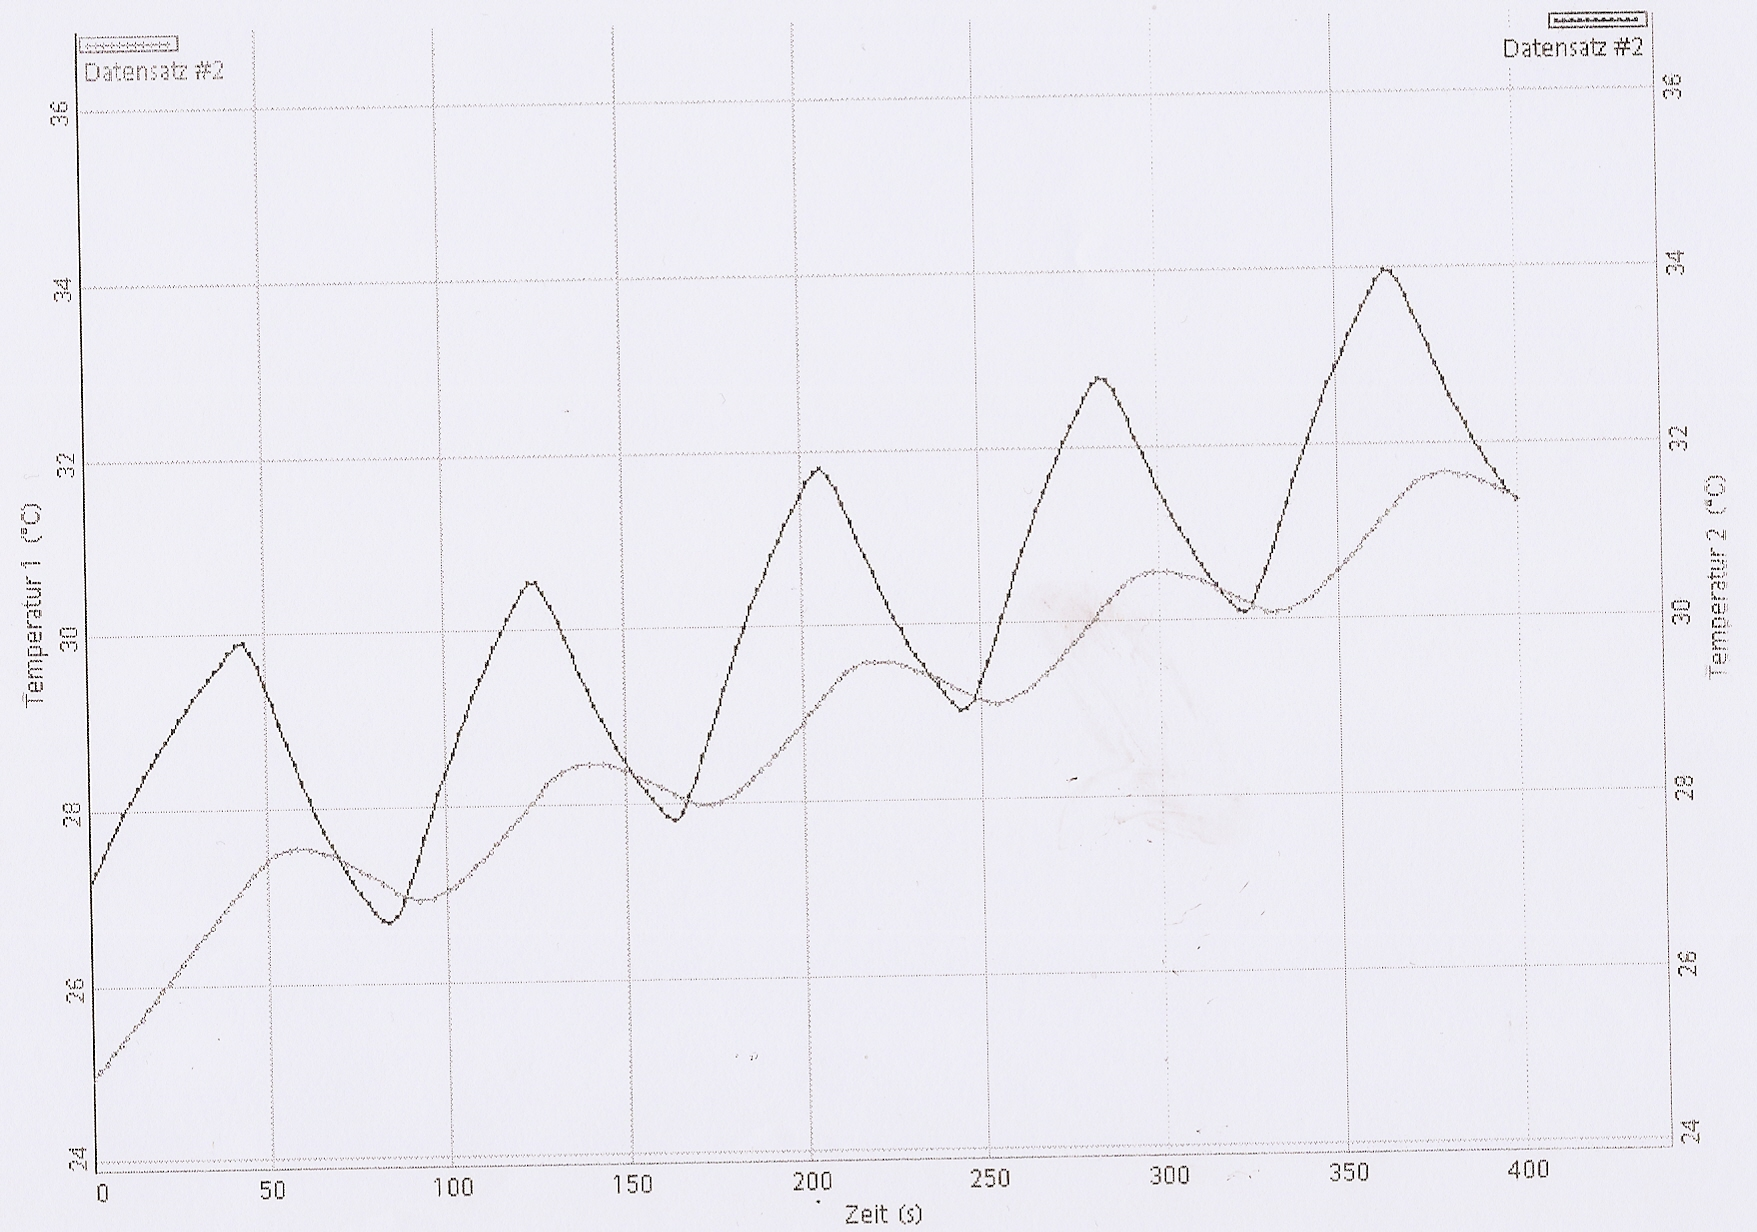
\includegraphics[height= 5cm, width = \textwidth]{logos/pT1.jpg}
    \caption{von Termoelement 1 und 2 (Messing, breit) bei einer Periode von 80s}
    \label{fig:pT12}
  \end{subfigure}
  \begin{subfigure}{0.48\textwidth}
    \centering
    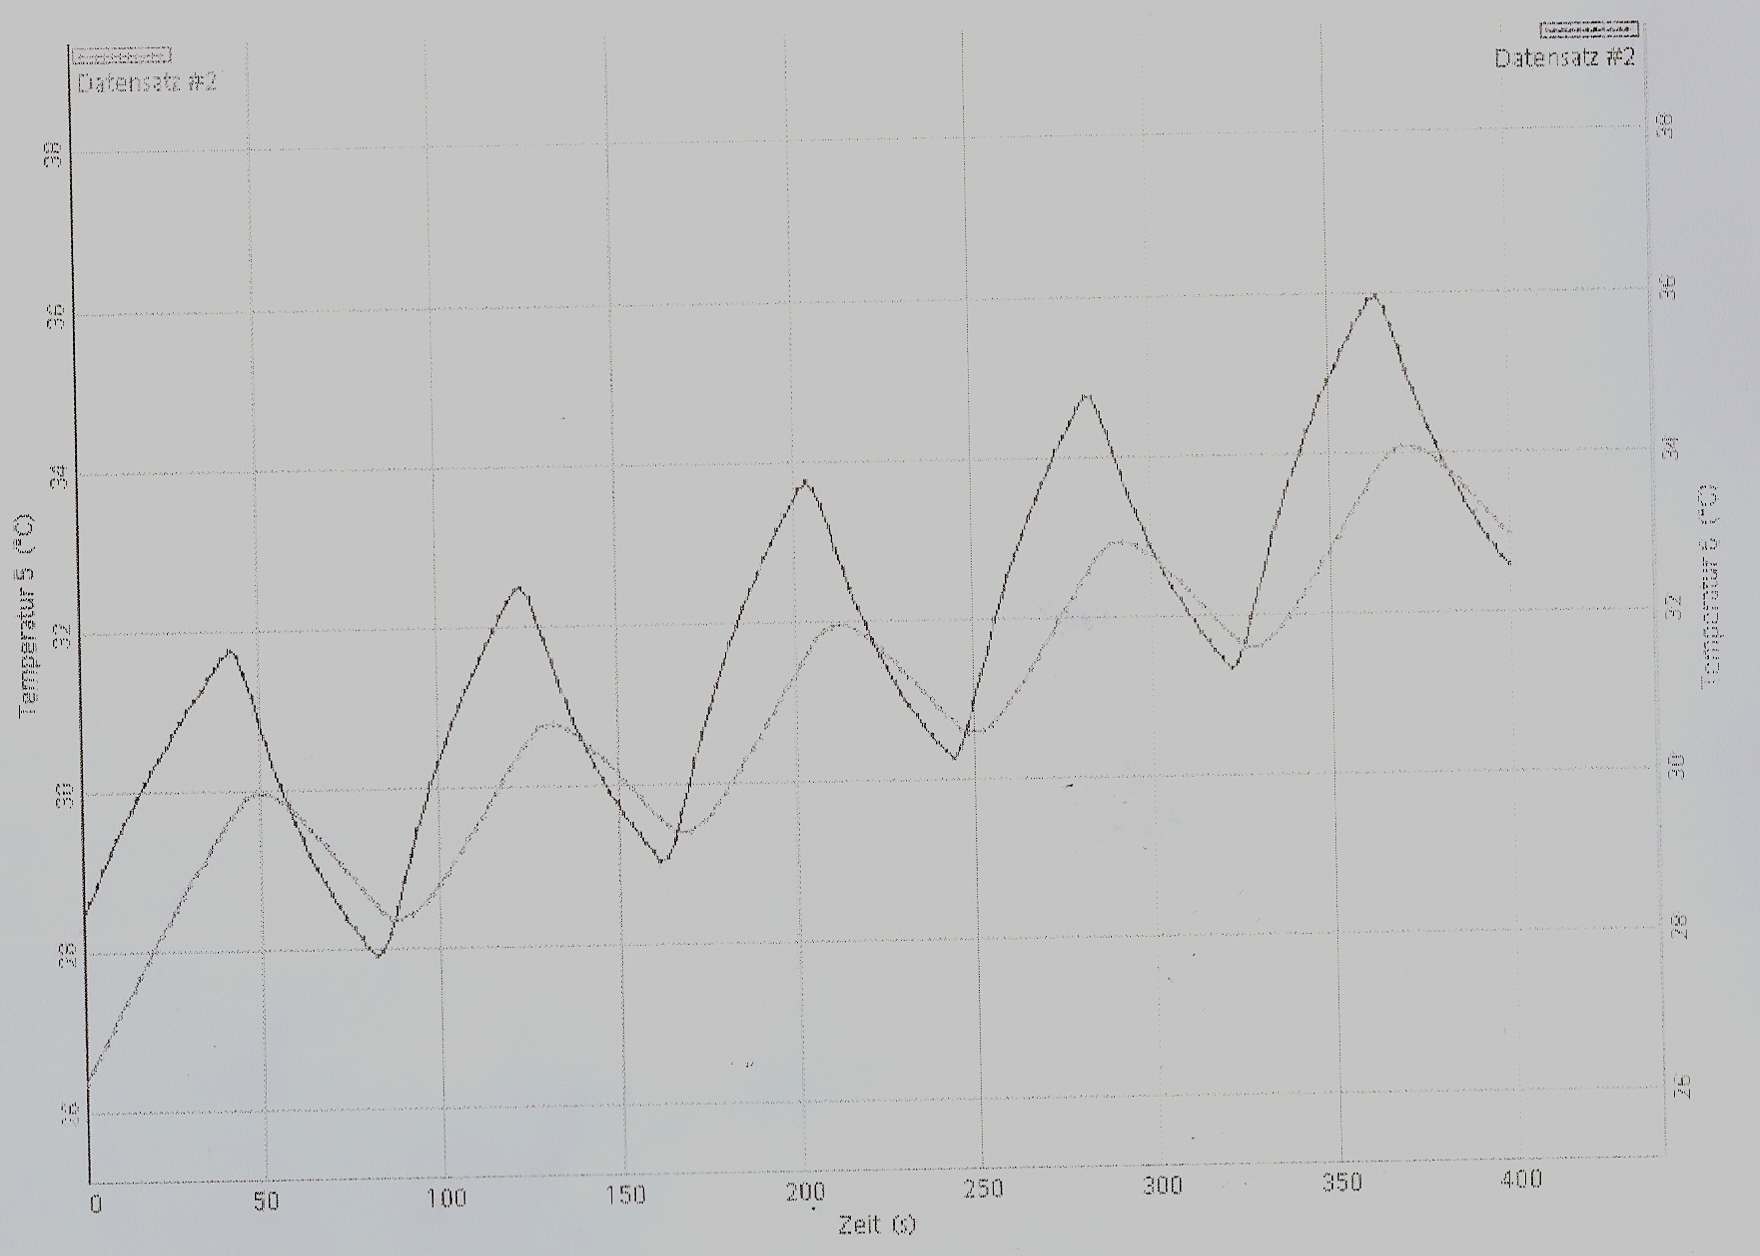
\includegraphics[height = 5cm , width = \textwidth]{logos/p40sT5.jpg}
    \caption{von Termoelement 5 und 6 (Aluminium) bei einer Periode von 80s}
    \label{fig:pT56}
  \end{subfigure}
  \\
  \begin{subfigure}{0.48\textwidth}
    \centering
    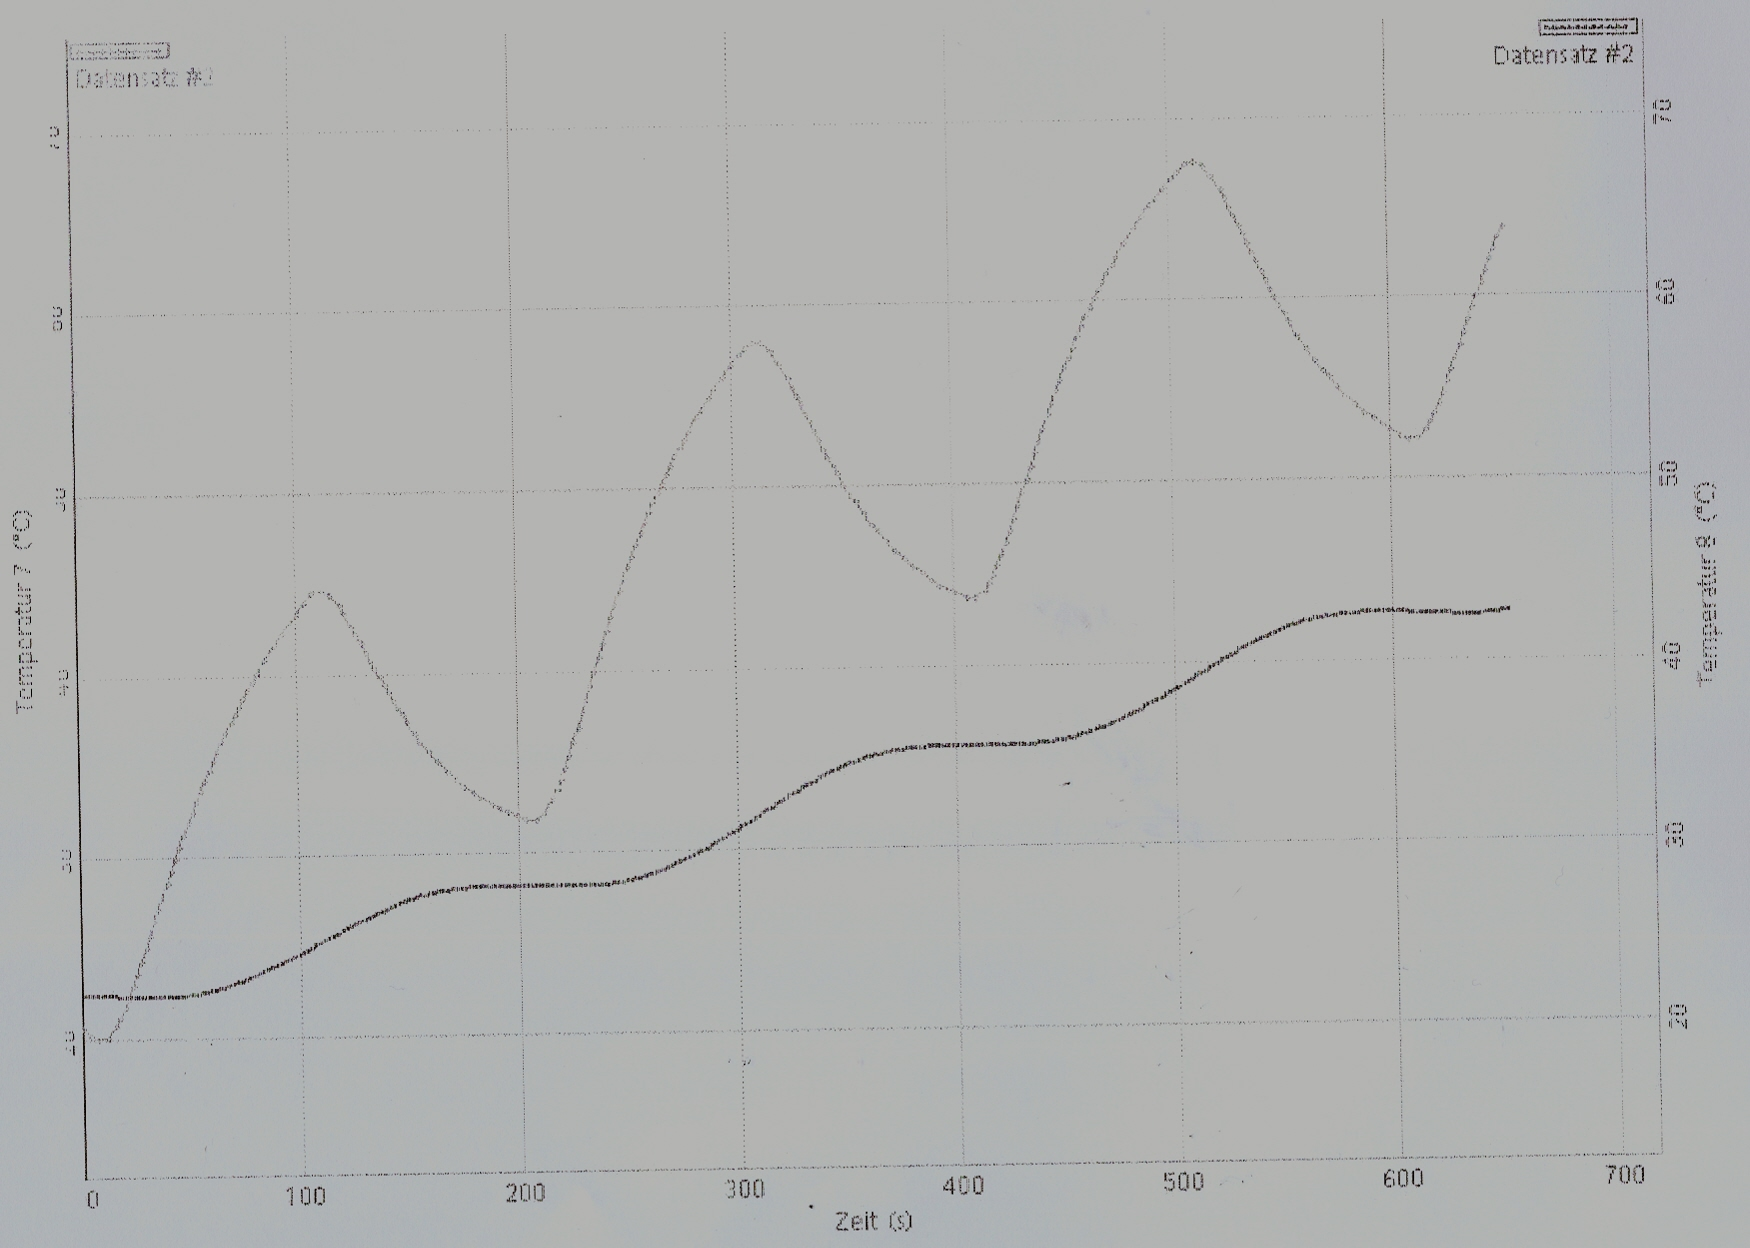
\includegraphics[height=5cm, width= \textwidth]{logos/pT7.jpg}
    \caption{von Termoelement 7 und 8 (Edelstahl) bei einer Periode von 200s}
    \label{fig:pT78}
  \end{subfigure}
  \label{fig:dfall}
\end{figure}
\begin{table}
  \centering
  \caption{Mittel der berechneten Wärmeleitfähigkeiten}
  \begin{tabular}{c c}
    \toprule
    Metal & $\kappa$/$\si{\watt\per\meter\per\kelvin}$ \\
    \midrule
    Messing & 117.35 \\
    Aluminium & 203.19 \\
    Edelstahl & 20.72 \\
    \bottomrule
  \end{tabular}
  \label{tab:kappa}
\end{table}
\FloatBarrier
Mit den Werten aus Abbildung \ref{fig:dfall} und
Tabelle \ref{tab:kappa} lässt sich mit
der Gleichung
\begin{equation*}
  v = \sqrt{\frac{2\kappa \omega}{\rho c }} \quad \text{mit} \quad
  \omega = 2\pi f = \frac{2\pi}{T}
  \quad \text{und} \quad
  \lambda = \frac{v}{f}
  \implies \lambda = \sqrt{\frac{4\pi\kappa}{f \rho c}}
\end{equation*}
die Wellenlänge $ \lambda $ der Temperaturwelle bestimmen. Dabei ist
$T$ die Periodendauer des Warm-Kalt-Wechsels der dynamischen Methode und
$v$ die Phasengeschwindigkeit der Temperaturwelle.
\begin{table}
  \centering
  \caption{Wellenlängen der Temperaturwellen}
  \begin{tabular}{cc}
    \toprule
    Metal & $\lambda$/\si{\meter} \\
    \midrule
    Messing & 0.19 \\
    Aluminium & 0.3 \\
    Edelstahl & 0.13 \\
    \bottomrule
  \end{tabular}
  \label{tab:lam}
\end{table}





























%
